\documentclass[11pt,a4paper]{article}

\usepackage[spanish,es-noquoting]{babel}
\usepackage[utf8]{inputenc}
\usepackage[T1]{fontenc}
\usepackage{lmodern}
\usepackage{geometry}
\usepackage{booktabs}
\usepackage{tabularx}
\usepackage{longtable}
\usepackage{array}
\usepackage{float}
\usepackage{graphicx}
\usepackage{enumitem}
\usepackage{hyperref}

\geometry{margin=2.5cm}
\setlength{\parskip}{0.6em}
\setlength{\parindent}{0pt}
\hypersetup{colorlinks=true, linkcolor=black, urlcolor=blue}

\title{Proyecto 2 - Data Mining\\\large Semana 2: Preparacion de Datos y Modelos Base}
\author{Javier Espana \and Angel Esquit \and Roberto Barreda \and Diego Lopez}
\date{Abril 2026}

\begin{document}

\maketitle

\begin{center}
Universidad del Valle de Guatemala\\
Curso: Data Mining\\
Dataset: Wisconsin Breast Cancer Dataset\\
Objetivo de clasificacion: \texttt{Class} (2 = Benigno, 4 = Maligno)
\end{center}

\hrule

\section{Objetivo de Semana 2}

Durante la Semana 2 se realizo la preparacion formal de datos, la seleccion de escenarios de variables y el entrenamiento de tres modelos base sin optimizacion de hiperparametros. Esta fase establecio la linea base para la comparacion posterior en Semana 3.

\section{Preprocesamiento de Datos}

\subsection{Limpieza del dataset}

El archivo \texttt{Datos.csv} contiene 683 registros originales y 11 columnas. Se aplicaron los siguientes pasos:

\begin{itemize}[leftmargin=1.2cm]
\item Eliminacion de 8 filas duplicadas.
\item Tratamiento de \texttt{Bare Nuclei}: los valores \texttt{"?"} se reemplazaron por nulos y se eliminaron las filas correspondientes.
\item Verificacion de rangos validos (1--10) en variables predictoras.
\item Exclusion de \texttt{Sample code number} por ser identificador no predictivo.
\end{itemize}

El dataset final para modelado (\texttt{Datos\_modelado.csv}) quedo en 675 registros, con 9 variables predictoras y la variable objetivo \texttt{Class}.

\subsection{Particion de datos}

Se utilizo particion \texttt{train/test = 80/20} estratificada con \texttt{random\_state = 42}, preservando la proporcion de clases en ambos conjuntos.

\begin{table}[H]
\centering
\caption{Distribucion de muestras por particion y clase}
\begin{tabular}{lccc}
\toprule
Particion & Total & Benigno (2) & Maligno (4) \\
\midrule
Entrenamiento & 540 & 351 (65.0\%) & 189 (35.0\%) \\
Prueba & 135 & 88 (65.2\%) & 47 (34.8\%) \\
\bottomrule
\end{tabular}
\end{table}

\section{Seleccion de Variables}

La variable objetivo fue \texttt{Class}. Se evaluaron dos escenarios:

\begin{itemize}[leftmargin=1.2cm]
\item \textbf{Escenario A:} las 9 caracteristicas citologicas disponibles.
\item \textbf{Escenario B:} top 3 variables con mayor correlacion con el diagnostico: \texttt{Bare Nuclei}, \texttt{Uniformity of Cell Size} y \texttt{Uniformity of Cell Shape}.
\end{itemize}

Se documento la multicolinealidad alta entre \texttt{Uniformity of Cell Size} y \texttt{Uniformity of Cell Shape} ($r = 0.91$), considerada un riesgo para modelos lineales sin regularizacion.

\textbf{Conexion explicita con Semana 1:} el Escenario B no es solo una reduccion por desempeno, sino una respuesta directa al hallazgo de colinealidad del EDA. Su objetivo fue medir si un subconjunto pequeno y altamente informativo podia sostener rendimiento con menor redundancia.

\textbf{Sobre PCA:} se considero PCA como alternativa de manejo de colinealidad, pero no se adopto en esta etapa por tres razones: (i) solo hay 9 variables originales, (ii) se priorizo interpretabilidad clinica de variables observables, y (iii) la estrategia L2 + comparacion A/B permitia controlar colinealidad sin perder trazabilidad de cada rasgo.

\section{Modelos Base}

Se entrenaron tres modelos sin tuning para establecer referencia comparativa.

\subsection{Regresion Logistica}

Modelo lineal de referencia para clasificacion binaria. Se aplico \texttt{StandardScaler}. La regularizacion L2 por defecto mitiga parcialmente el efecto de multicolinealidad y permite interpretacion directa de coeficientes.

Esta configuracion se uso deliberadamente como respuesta tecnica al riesgo de colinealidad identificado en Semana 1.

\subsection{KNN (k = 5)}

Clasificador basado en vecinos mas cercanos, sin supuestos de linealidad en la frontera de decision. Requiere escalado de variables y se utilizo \texttt{k=5} como baseline.

\subsection{SVM con kernel RBF}

Modelo no lineal basado en maximizacion de margen con kernel RBF. Se eligio por la separabilidad observada en el EDA y su robustez relativa frente a outliers. Parametros base: \texttt{C=1.0} y \texttt{gamma="scale"}.

\section{Resultados y Comparacion}

\subsection{Escenario A: Todas las variables}

Las metricas se reportan para la clase positiva (maligna).

\begin{table}[H]
\centering
\caption{Metricas de modelos base en Escenario A}
\begin{tabular}{lcccc}
\toprule
Modelo & Accuracy & Precision & Recall & F1-Score \\
\midrule
Regresion Logistica & 0.9556 & 0.9362 & 0.9362 & 0.9362 \\
KNN (k=5) & 0.9556 & 0.9362 & 0.9362 & 0.9362 \\
SVM (RBF) & 0.9630 & 0.9375 & 0.9574 & 0.9474 \\
\bottomrule
\end{tabular}
\end{table}

\begin{table}[H]
\centering
\caption{Matrices de confusion en Escenario A (FN = falsos negativos)}
\begin{tabular}{lccccc}
\toprule
Modelo & TN & FP & FN & TP & Recall \\
\midrule
Regresion Logistica & 85 & 3 & 3 & 44 & 0.9362 \\
KNN (k=5) & 85 & 3 & 3 & 44 & 0.9362 \\
SVM (RBF) & 85 & 3 & 2 & 45 & 0.9574 \\
\bottomrule
\end{tabular}
\end{table}

En este escenario, SVM supero a LR y KNN en recall y en reduccion de falsos negativos.

\begin{figure}[H]
\centering
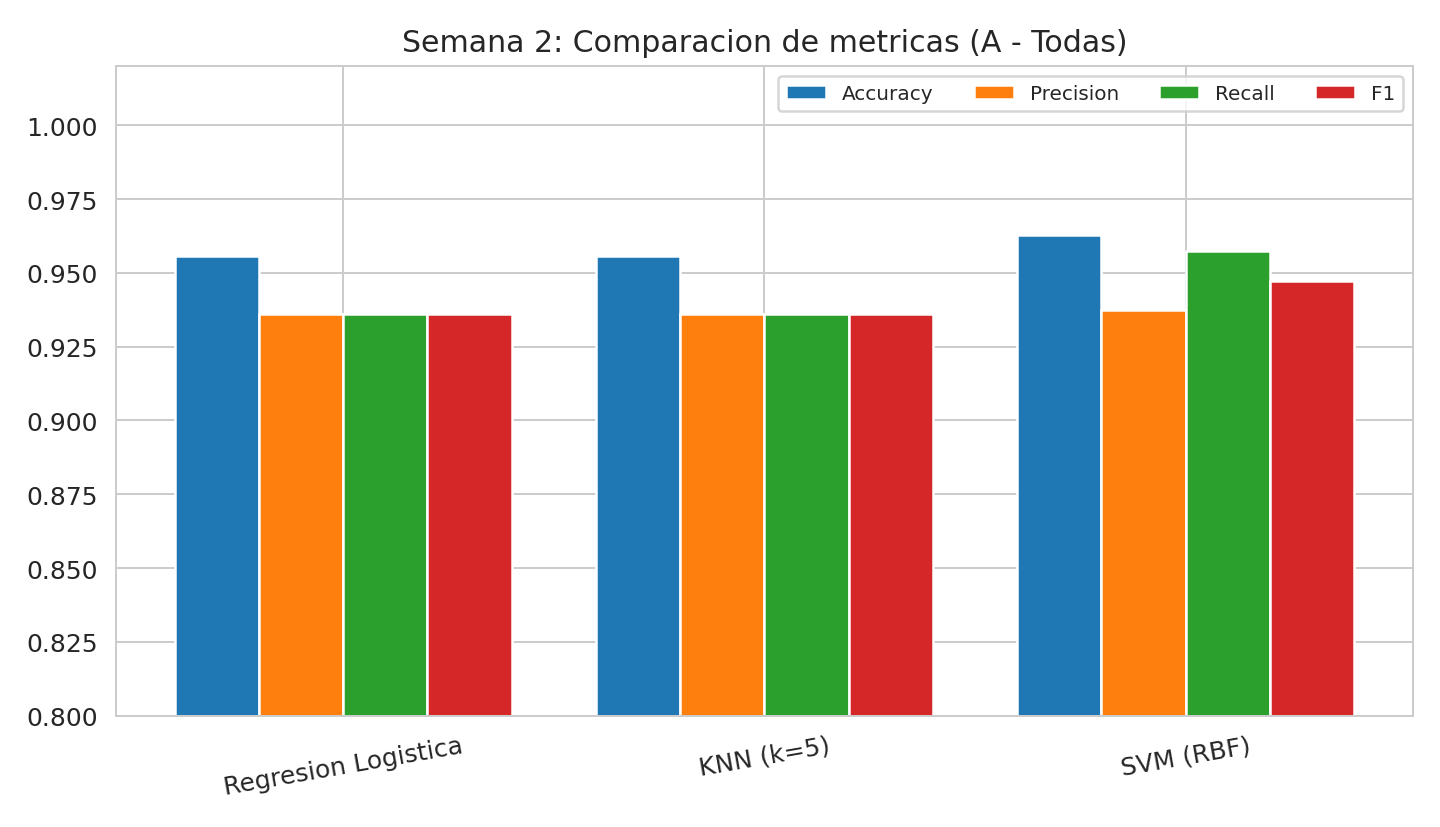
\includegraphics[width=0.9\textwidth]{figures/s2_metricas_A.png}
\caption{Comparacion visual de metricas de modelos base en Escenario A.}
\end{figure}

\subsection{Escenario B: Top 3 variables}

\begin{table}[H]
\centering
\caption{Metricas de modelos base en Escenario B}
\begin{tabular}{lcccc}
\toprule
Modelo & Accuracy & Precision & Recall & F1-Score \\
\midrule
Regresion Logistica & 0.9259 & 0.9302 & 0.8511 & 0.8889 \\
KNN (k=5) & 0.9481 & 0.9348 & 0.9149 & 0.9247 \\
SVM (RBF) & 0.9481 & 0.9348 & 0.9149 & 0.9247 \\
\bottomrule
\end{tabular}
\end{table}

Al reducir variables, LR se degrada de forma mas marcada en recall, mientras que KNN y SVM muestran mayor robustez.

\begin{figure}[H]
\centering
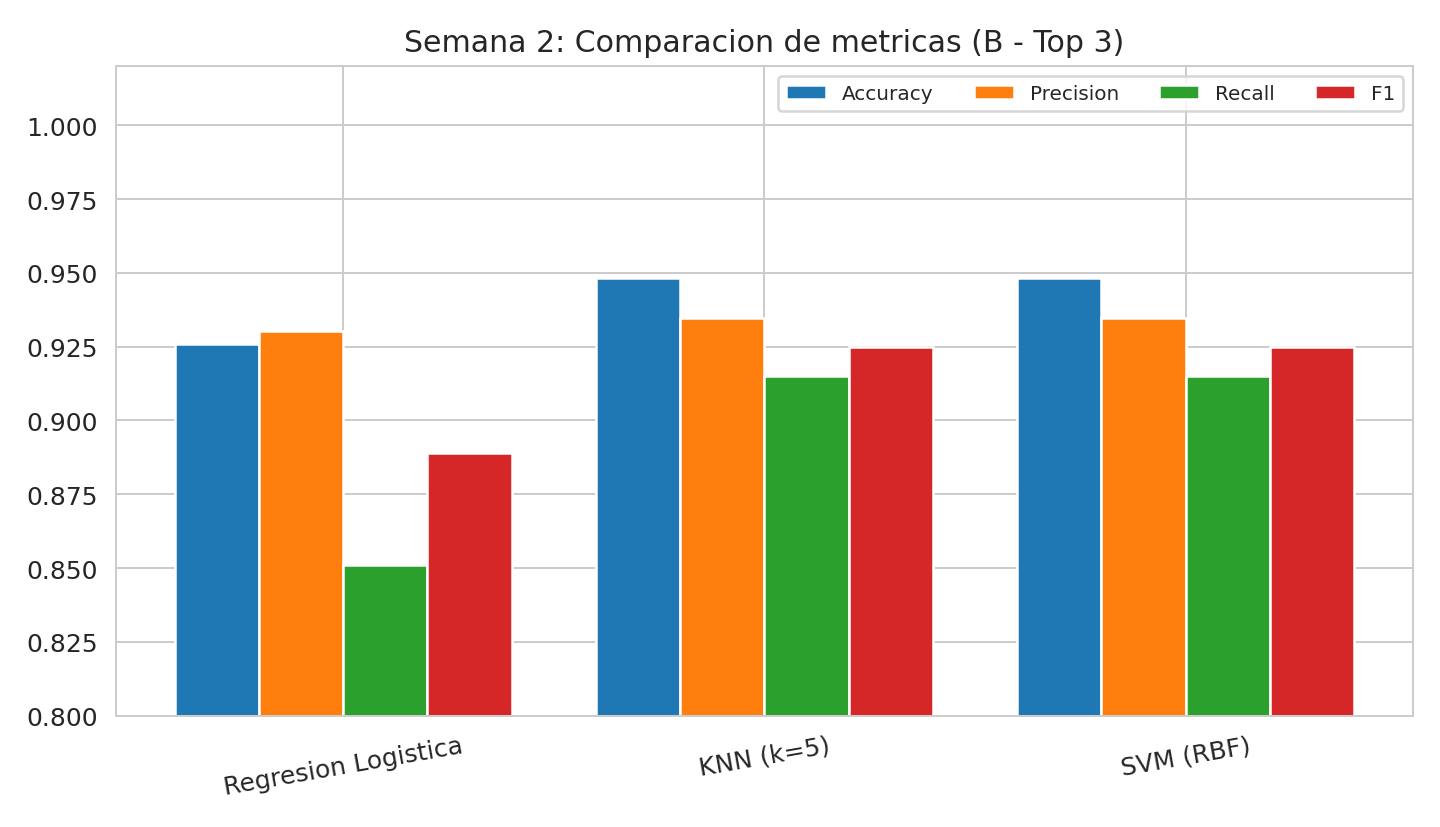
\includegraphics[width=0.9\textwidth]{figures/s2_metricas_B.png}
\caption{Comparacion visual de metricas de modelos base en Escenario B.}
\end{figure}

\subsection{Lectura comparativa A vs B}

Al pasar de A a B se observa un patron claro:

\begin{itemize}[leftmargin=1.2cm]
\item En LR, la reduccion de variables provoca la mayor caida de sensibilidad en clase maligna.
\item En KNN y SVM, el deterioro es menor, lo que sugiere mayor robustez ante compresion del espacio de variables.
\item El mejor baseline global sigue estando en Escenario A, lo que justifica que la optimizacion de Semana 3 priorice ese escenario para la seleccion final.
\end{itemize}

\section{Conclusiones Iniciales}

\begin{enumerate}[leftmargin=1.2cm]
\item El mejor modelo base fue \textbf{SVM con kernel RBF} en Escenario A, por mayor recall y menor FN.
\item Regresion Logistica y KNN empataron en Escenario A, quedando como candidatos competitivos.
\item LR mantiene ventaja interpretativa por coeficientes, aunque pierde robustez al reducir variables.
\item KNN y SVM fueron mas robustos que LR en Escenario B.
\item Se confirma la hipotesis H3 de Semana 1: recall de clase maligna como metrica prioritaria.
\item La hipotesis H4 se abordo explicitamente con regularizacion L2 en LR y con el diseno de Escenario B como prueba de robustez ante colinealidad.
\item Aunque PCA era viable tecnicamente, se decidio no usarlo para conservar interpretabilidad de variables clinicas y porque el rendimiento obtenido con A/B + L2 fue suficiente para pasar a optimizacion.
\end{enumerate}

\section{Ajustes aplicados por retroalimentacion}

Con respecto a los errores de narrativa de la version previa, esta semana queda corregida en tres puntos:

\begin{enumerate}[leftmargin=1.2cm]
\item Se conecta explicitamente el \textbf{Escenario B} con el hallazgo de colinealidad de Semana 1.
\item Se documenta la decision metodologica sobre \textbf{PCA} (evaluado y no adoptado en esta fase).
\item Se deja trazabilidad de que la \textbf{regularizacion L2 en LR} se uso como respuesta tecnica a la colinealidad identificada en el EDA.
\end{enumerate}

\section{Anexo}

Repositorio del proyecto:\\
\url{https://github.com/AngelEsquit/PRY2-MD.git}

\end{document}
